\documentclass[a4paper,fontsize=10pt,twoside,DIV15,BCOR12mm,headinclude=true,footinclude=false,pagesize,bibtotoc]{scrbook}


\usepackage{pslatex} % -- times instead of computer modern, especially for the plain article class
\usepackage[colorlinks=false,bookmarks=false]{hyperref}
\usepackage{booktabs}
\usepackage{graphicx}
\usepackage{xcolor}
\usepackage{multirow}
\usepackage{cite}
%\usepackage{flushend} % even out the last page, but use only at the end when there is a bibliography

\newcommand{\code}[1]{{\small{\texttt{#1}}}}

% fatter TT font
\renewcommand*\ttdefault{txtt}
% another TT, suggested by Alex
% \usepackage{inconsolata}
% \usepackage[T1]{fontenc} % needed as well?

\usepackage{listings}

\newcommand{\todo}[1]{{\emph{TODO: #1}}}
\newcommand{\martin}[1]{{\color{blue} Martin: #1}}
\newcommand{\morten}[1]{{\color{red} Morten: #1}}

% uncomment following for final submission
%\renewcommand{\todo}[1]{}
%\renewcommand{\martin}[1]{}
%\renewcommand{\author2}[1]{}

\begin{document}

\title{Leros: the Return of the Accumulator Machine}

\author{Martin Schoeberl and Morten Borup Petersen}

\lowertitleback{Copyright \copyright{} 2018 Technical University of Denmark
  \medskip\\
  \begin{tabular}{lp{.8\textwidth}}
    \raisebox{-12pt}{
\includegraphics[height=18pt]{fig/cc_by_sa}} &
     This work is licensed under a Creative Commons Attribution-ShareAlike
     4.0 International License.
     \url{http://creativecommons.org/licenses/by-sa/4.0/}\\
  \end{tabular}
}

\frontmatter

\maketitle

\chapter{Preface}

This handbook shall evolve to the documentation of the Lerso processor and the
Leros compiler. In the mean time it is intended to collect design notes and discussions.

This document shall evolve into three different document: (1) a handbook for Leros,
(2) Morten's BA thesis, and (3) a journal article on Leros and the compiler.

Leros is a tiny microcontroller that is optimized for current low-cost FPGAs. Leros is designed with a balanced logic to on-chip memory relation. The design goal is a microcontroller that can be clocked in about half of the speed a pipelined on-chip memory and consuming less than xxx logic cells.

The architecture, which follows from the design goals, is a pipelined 16/32/64-bit accumulator processor. An implementation of Leros needs at least one on-chip memory block and a few hundred logic cells.

The application areas of Leros are twofold: First, it can be used as an intelligent peripheral device for auxiliary functions in an FPGA based system-on-chip design. Second, the very small size of Leros makes it an attractive softcore for manycore research with low-cost FPGAs.

\section{Notes}

Here collect of notes and ideas in bullet list for the development and writing process:

\begin{itemize}
\item Collect related work
\item Some more notes
\item We shall have some calling and usage convention, we have very many register so we can have
stuff like pointer to (larger) constants
\end{itemize}

Leros 1 has been forked and extended: \url{https://github.com/jonpry/leros}.

\subsection{Mortens notes (ISA, compiler related)}
\begin{itemize}
\item Does it make sense to set the immediate/register selector bit to 1 (immediate) in a store instruction?
\martin{no}
\item What is the final descision on loadh4/5/6/7 opcodes for Leros64?
\item We emit small inline algorithms for stuff such as: test-and-set, sra, lsh, sign-extension
\item what is the sense of the argument to the shr instruction? is shr with a register operand loading a register, right-shifting the value by 1 and storing it in the accumulator?
\martin{no, this is all ignored. Yes, we waste some instruction bits. Therefore, encoding should be rethought.}
\item and/or/xor: When these instructions have immediate values, is the logical operation masked for the lower 8-bits of the accumulator? as in, the remaining upper bits of the accumulator remains untouched.
\martin{In the original implementation of Leros, the immediate value is sign extended before arithmetic \emph{and}
logic operations. Questionable.}
\morten{From a normal point of view I think sign-extension for all arithmetic instructions makes sense, but not for logic operations, since the semantics of the extended bits change, based on the logical operation - ie. sign-extending an 8-bit bitmask for AND with 1 as MSB will not be semantically equivalent to sign-extending the same bitmask for OR, which might lead to some dangerous/unhandled situations. BUT I do recognize the value of it, as the non-discrepancy allows for a smaller hardware footprint. It is mainly a question of whether the compiler should factor in sign-extension when generating bitmasks. Factoring in sign extension is already implemented into immediate loading, and the only places where bitmasks are currently generated are in sign-extended loads. If this is the operation of the logical operations with immediates, i of course have to factor this in to all accumulator-immediate logical operations upon instruction emission.}
\martin{I agree. I should probably simply cut the connection to the original Leros implementation in order to free our
minds for better architectural decisions.}
\item \morten{Branch offset:} Currently, branch offsets can be specified as a regular 8-bit immediate. This gives us an effective PC-relative branch target range of +-128 bytes which is +-64 instructions. Now, this is a very small range, and i fear that with the emmission of the small algorithms for ie. select, shift, etc. instructions, a range of 64 instructions could potentially render branch instructions quite useless. To rememdy this, we could do as ie. RISC-V, and assume that bit 0 of the branch target always is 0, effectively doubling our branch target range to +-128 instructions. This would also make sense, since we do not need to be able to branch 8-bit aligned adresses - instructions will always be 16-bit aligned.
\martin{Yes, sure. This has been always the idea in Leros. We do not waste branch offset bits for
unusable target addresses. This is usually done, it is not only a RISC-V feature.}
Now, implementing this in the current datapath of the processor does not seem to be viable, since we do not have left-shift hardware, and thus are unable to interpret an 8-bit immediate as a 9-bit immediate with b0=0. 
\martin{Hey, hey! Left shift by a constant in the data path is for free. It is only redefining wires.
No hardware needed here.}
This might be a motivation for adding a left-shift by 1 instruction and the accompanying hardware. 
Another option could be to assume that the two lower-most bits of a branch target is zero (thus, branch targets are always 32-bit aligned), and gaining a pc-relative branch range of +-256 instructions. Then, from the compiler, we could make sure that basic-blocks are always 32-bit aligned, and pad with a 'nop' instruction if this is seen to not be the case. 
Thoughts?
\martin{Yes, this could be explored. Although small code fragments (if/else, small loops) may introduce
quite some overhead (of 1/2 and instruction).
An additional option is to use more than 8 bits of the instruction for branches. We have quite some
space in the instruction encoding. The same issue could be discussed for immediate constants.
I hope we can have some interesting discussion/writing on those tradeoffs in this document.}
\item \morten{I was wondering about the PC register in the Leros processor. Is this synthesized to be 31 or 32 bits long? I assume that it could be inferred to be 31 bits long since we always assume that instructions are halfword aligned.}
\martin{Yes, that is a common ``optimization'' I usually do. But I slowly change my mind that this thinking in
words or halfwords for the PC is really not worth the optimization of 1 or 2 bits.}
\end{itemize}

\subsection{Using LLVM for atypical architectures (stack/accumulator/etc. based - everything thats not 3-operand ISAs)}
\begin{itemize}
\item The LLVM IR is pattern matched to an an intermediate wrapper-ISA of the target architecture - could be called a pseudo-ISA. This Pseudo-ISA is a wrapper for all of the implemented instructions in the target ISA, but with a 3-operand type signature. With this, the LLVM backend can work with the ISA as intended, in relation to register allocation, schedueling, liveness tracking etc.

\item There are obvious drawbacks to this - many redundant loads and stores will be produced, default schedueling will schedule unaware of the accumulator, and suboptimal codesequences can be selected. The main benefit is, that we by doing this can use the LLVM backend as-intended - ie. for 3-operand ISAs, as well as creating semantically correct code. So for having a prototyping compiler, one in which semantical correctness and good-enough code is produced, this is an acceptable method, since it allows for a fairly quick implementation time. 
\item The pseudo-ISA also helps us in other ways - some instructions are from LLVMs point of view expected to be available in the target ISA, and as such are hard to expand to other sequences of instructions before instruction selection. In LLVM this is set by setOperationAction() where we specify what to do when encountering an LLVM SD node of said type. Usually, it is actions such as multiplication etc., which are expected to be expanded to longer sequences - llvm is built for this. But for operations such as shifts, it is expected that the target ISA implements this. Here, we utilize the pseudo ISA to match these actions (since we are unable to expand them pre-instruction selection), and during instruction emission, mark these pseudo instructions as having custom emitters (see EmitInstrWithCustomInserter) 
\end{itemize}

\subsection{Questions to be Answered by Compiling Example Programs}

\begin{itemize}
\item We should be relaxed on compatibility with Leros 1. It is nor widely used, so we can move on
with incompatible changes. Just keep the spirit of the original Leros design.
\item Cost/benefit of: 
\begin{itemize}
    \item arithmetic shift right
    \item compare and set (setCC in llvm)
    \item Unsigned comparison frequency
\end{itemize}
\item With tighter encoding we could have up to a 15-bit constant and/or wider branches
\item constant pool lowering; oftentimes build masks in custom emissions - these should be placed in a constant pool.
\item 
\item 
\item 
\end{itemize}

\subsection{Questions to be Answered by Hardware Experiments}

\begin{itemize}
\item Cost \emph{sloppier} encoding. Is it worth to have the immediate bit in one place?
\item How to build a fast ALU. This will still be the critical path if done sloppy.
\item 
\item 
\item 
\item 
\end{itemize}

\subsection{ALU Experiments}

Just take notes here for now. This would probably better placed in the Chisel digital design
book.

Experiments are based on DE2-115 setup (EP4CE115F29C7, slow timing at 85 C).
Compiler: Performance, aggressive.

Pain ALU with function as number (Enum), +, -, or, and, xor, ld, shr, and nop. Plus enable:
fmax = 199 MHz, design distributed over 3 LABs

+, -, keep, and enable: 117 LCs (probably add, sub, and mux), distributed over 4 LABs, fmax = 219 MHz

+, keep, and enable: still 100 LCs, fmax = 226 MHz

Baseline: just an unconditional +: 32 LCs, still distributed over 3 LABs, fmax = 261 MHz

Variations of adding: 31 bits: 262 MHz, 30 bits 269 MHz, 28 bits 279 MHz, 16 bits 363 MHz, 64 bits 171 MHz

Baseline logic: just an OR function: 1142 MHz

Logic AND and OR with mux, should fit into on LC, resource are 43 LCs (some for decode, ok), fmax 449 MHz

Looks like aiming for 200 MHz is challenging enough, as we need some more MUXs
for various loads.



\chapter{Introduction}
\label{sec:intro}

Instruction set design has been considered uninteresting or less important for computer
architecture in the last decades~\cite{the right H and P book, or the slides}.
However, the recent work on RISC-V was even worth a full PhD for the ISA design
for a RISC type architecture~\cite{Andrew thesis}.
The very same people considering ISAs uninteresting are reestablishing work on
designing the \emph{right} RISC instruction set.

We agree on the idea of rethinking ISA design within the change of technology.
When processor pipelines are primarily waiting for memory accesses, the design
tradeoffs for an ISA may be different than some decades ago.
Old architectures, such as accumulator machines or stack machines, may be worth
to be reconsidered.

There are initiatives of ISA that are very minimal, such as the single instruction
processor~\cite{find it}. Although it is Touring complete, \martin{Is it?} we consider this
an obscure architecture.
We aim at a minimal and useful ISA, whatever this means.

With Leros we present an accumulator machine ISA that takes advantage of cheap
on-chip memory for a large register file and being aware of possible very high cost
of access to main memory (and IO devices).


In this paper we present Leros, a microcontroller that is optimized for low-cost FPGAs.
Leros is a minimalistic 16/32/64-bit processor intended for utility functions in an FPGA based
system-on-chip design. The design goals of Leros are a good balance between
the number of logic cells and on-chip memories, reasonable performance, and a high
maximum clock frequency. The last point is important for usage as utility processor
in an SoC to not be the frequency bottleneck of the whole design.

These design goals are achievable by a pipelined accumulator architecture with
additional directly addressable \emph{registers} in an on-chip memory for local variables.
The on-chip data memory is shared for those registers and general data.
With an additional on-chip memory for the instructions only two memory blocks are
needed and the pipeline can execute one instruction per clock cycle.
For short programs the instruction memory can even be built out of logic cells (LC).

Leros is named after the greek island Leros,\footnote{\url{http://www.leros.gr/}}
where it has been designed during an enjoyable vacation. Leros is available
under open-source and if you use Leros in your application or research,
consider a visit to the nice island Leros and sending a postcard from there to the authors.

\todo{Most text is a copy from the original Leros paper~\cite{leros:fpl2011} and needs
to be rewritten. The original Leros has also been used for an embedded JVM~\cite{leros:jvm}.}

This paper... \todo{purpose statement, latest in 4th paragraph}

\todo{Test the bib with a reference that gives background on time-predictable
computer architecture~\cite{tpca:jes}.}

A paper is cited \cite{paper:example}.

The contributions of this paper are: (1) ... (2) ...

This paper is organized in N sections: The following section presents related work.
Section~\ref{sec:background} provides background on ...
Section X and Y 
Section~\ref{sec:eval} evaluates...
Section~\ref{sec:conclusion} concludes.

\chapter{Related Work}
\label{sec:related}

\todo{Show that you know the field. All related work shall be put
into context or contrast to our current work.}



\chapter{Instruction Set Architecture}
 
 Leros is a 16/32-bit architecture with 16-bit instructions and 16/32/64-bit data.
 In an accumulator design the addresses of one source operand and the destination are implicit.
 Therefore, only one operand (address) needs to be encoded in the instruction.
 Furthermore, this relaxed instruction encoding allows for 8-bit immediate values in the instruction.
 The common ALU operations are supported with one operand from the register area (256 words)
 in the data memory or with an 8-bit immediate value.
 The data memory can be accessed via indirect loads and stores.
 \todo{more details on the split address/load/store? Perhaps in the implementation section.} I/O ports are accessed with dedicated instructions and an 8-bit address.
  
Conditional and unconditional branches use 8 bit relative offsets.
For longer jump destinations, function calls, return from a function call, and computed jump
destinations an indirect jump via the address in the accumulator is supported (jump-and-link).
The jump-and-link instruction saves the program counter into a register.


The instructions of Leros can be categorized into following types:

    ALU operation with the accumulator and an immediate
    ALU operation with the accumulator and a register
    Load and store
    Indirect load and store
    Conditional branches
    Jump and link
    Shift right
    Input and output

Encoding

Instructions are 16 bits wide. The higher byte is used to encode the instruction, the lower byte contains either an immediate value, a register number, or a branch offset.

\begin{verbatim}
+--------+--------+
|iiiiiiii|nnnnnnnn|
+--------+--------+
\end{verbatim}



For example 00001001.00000010 is an add immediate instruction that adds 2 to the accumulator, where 00001000.00000011 adds the content of R3 to the accumulator. For branches we use 4 of the instruction bits
for larger offsets.

\section{List of Instructions}

Following table shows all currently defined instructions (21, if you include all conditional branch variations).

Not all instruction bits are currently used (unused are marked with -). Bit 0 selects between immediate and using a register. The following list is the complete instruction set.

\begin{verbatim}
+--------+----------+
|00000---| nop      |
|000010-0| add      |
|000010-1| addi     |
|000011-0| sub      |
|000011-1| subi     |
|00010---| shr      |
|00011---| -        |
|00100000| load     |
|00100001| loadi    |
|00100010| and      |
|00100011| andi     |
|00100100| or       |
|00100101| ori      |
|00100110| xor      |
|00100111| xori     |
|00101001| loadhi   |
|00101010| loadh2i  |
|00101011| loadh3i  |
|00110---| store    |
|001110-?| out      |
|000001-?| in       |
|01000---| jal      |
|01001---| -        |
|01010---| ldaddr   |
|01100-00| ldind    |
|01100-01| ldindb   |
|01100-10| ldindh   |
|01110-00| stind    |
|01110-01| stindb   |
|01110-10| stindh   |
|1000nnnn| br       |
|1001nnnn| brz      |
|1010nnnn| brnz     |
|1011nnnn| brp      |
|1100nnnn| brn      |
|11111111| scall    |
+--------+----------+
\end{verbatim}

\section{Comments}

loadh makes only sense for immediate values. For 32 bits we just need two more immediate loads, could simply by as follows:

Can easily be extended to 64 bits when ignoring the immediate bit. Load function from ALU could be dropped.

Load address and following load/store should be emitted as pair as they are dependent. Possible interrupts should be disabled between those two instructions.

\section{ISA Discussions}

\todo{We should have a discussion of the ISA and the rationale of decisions.}

These observations should be explored with a quantitative approach~\cite{H and P} by experiments
with real benchmarks, different compiler backends, and different pipeline implementations in
an FPGA.

\subsection{Branch Offsets and Immediate Values}

The initial design of the Leros ISA uses 16-bit instructions, where 8 bits are used for the
instruction encoding and 8 bits for an operand (register number of immediate). For branches
those 8 bist offsets result in a branch distance of around +/- 127 instructions.
The question is, if some more bits from the instruction encoding shall be spent for
branch offsets.



Similar to branch offsets are immediate values. With the initial encoding small immediate
values can be encoded very efficiently. However, a 32-bit constant may consume up to 4
instructions to be loaded. Would it make sense to use some of the instruction encoding space
to be able to load some 32-bit constants in only 3 instructions. Is it worth it? How many of those
constants do exists.

Furthermore, constants can also be loaded into a memory region and then loaded indirectly,
similar to the constant pool in the Java virtual machine. And some often used constants can
be allocated in one of the many (256) registers.

\subsection{Compare}

Compare instructions setting the result in the accumulator might make sense. The cost is not
the ALU, but the additional mux in the time critical path in the accumulator.

\subsection{IO}

IO operations can be implemented as \emph{normal} memory locations or as special IO instructions.
Currently we use the second approach with 8 bits for addresses, which might look very restrictive.
However, this restriction can always be resolved with \emph{another indirection}, which means writing
an effective IO device address first into one of the limited IO addresses. This additional instruction and
the timing is not really an issue, as IO operations are not so frequent.
Taking that observation to the next point is why should we have \emph{primary} IO addresses in
instructions in the first place. Maybe having just three IO operations: (1) write IO address, (2) read,
and (3) write.

The same observation is true for memory accesses. However, that step has already been designed
into the ISA of Leros with usage of an address register. One more argument to use the same mechanism
fo IO. Maybe the memory address register is also the one to be used for IO instructions.
In that case we could reconsider merging the memory and IO address space and use the same
load and store instructions for memory and IO access. One of the main issues is to keep those
load instructions out of the critical path of a pipeline implementation. An additional instruction/cycle
for a memory or IO operation is a minor issue.



\chapter{Leros Design Decisions}
\label{sec:design}

\section{New Aims}

An accumulator machine needs more instructions than a standard RISC architecture.
On the program size side, an accumulator machine can easily use just 16-bit instructions
instead of the typical 32-bit instructions for a RISC processor.

We also aim for a higher clock frequency then a 5-stage RISC pipeline. First, with an
accumulator design we avoid the forwarding network, that usually is in the critical path.
Furthermore, with less instructions, the ALU will be simpler as well.

One question is how many stages a pipeline shall have? Two or three stages seem practical.
The original Leros design had two stages: (1) fetch and decode and (2) register read and execute.
Our aim is at least double the frequency of a RISC pipeline. In the Cyclone~IV
Patmos can run at 80~MHz. So the very minimum would be 160~MHz.
Better towards 250~MHz. A Cyclone~IV memory can be clocked at 315~MHz.
Therefore, with full pipelining (4 stages) 300~MHz would be achievable.

Possible pipeline organizations:

\begin{description}
\item[2 stages:] (1) fetch and decode and (2) register read and execute
\item[3 stages:] (1) fetch and decode, (2) register read, and (3) execute
\item[3 stages:] (1) fetch, (2) decode and register read, and (3) execute
\item[4 stages:] (1) fetch, (2) decode, (3) register read, and (4) execute
\end{description}
\todo{Check how fast a NIOS can be clocked.}

\todo{Do we have an issue with a use after store? I think so. Not a very common combination, except
for the shift left.}

Main aims for an FPGA implementation (in the Cyclone~IV):

\begin{itemize}
\item less than 500 LCs
\item more than 250 MHz
\item 64 cores in the DE2-115
\item Readable Chisel code as example for the Chisel book
\end{itemize}


\section{Original Design Decisions}

To optimize a tiny processor core we evaluate the relation of on-chip memories to logic resources on current low-cost FPGAs. Furthermore, the maximum clock frequency of Leros shall be high enough to not constraint the overall maximum clock frequency of an SoC, where Leros is used as an intelligent peripheral device. We aim for a clock frequency half of the frequency of on-chip memories with input and output registers.


\begin{figure*}[t]
    \centering
    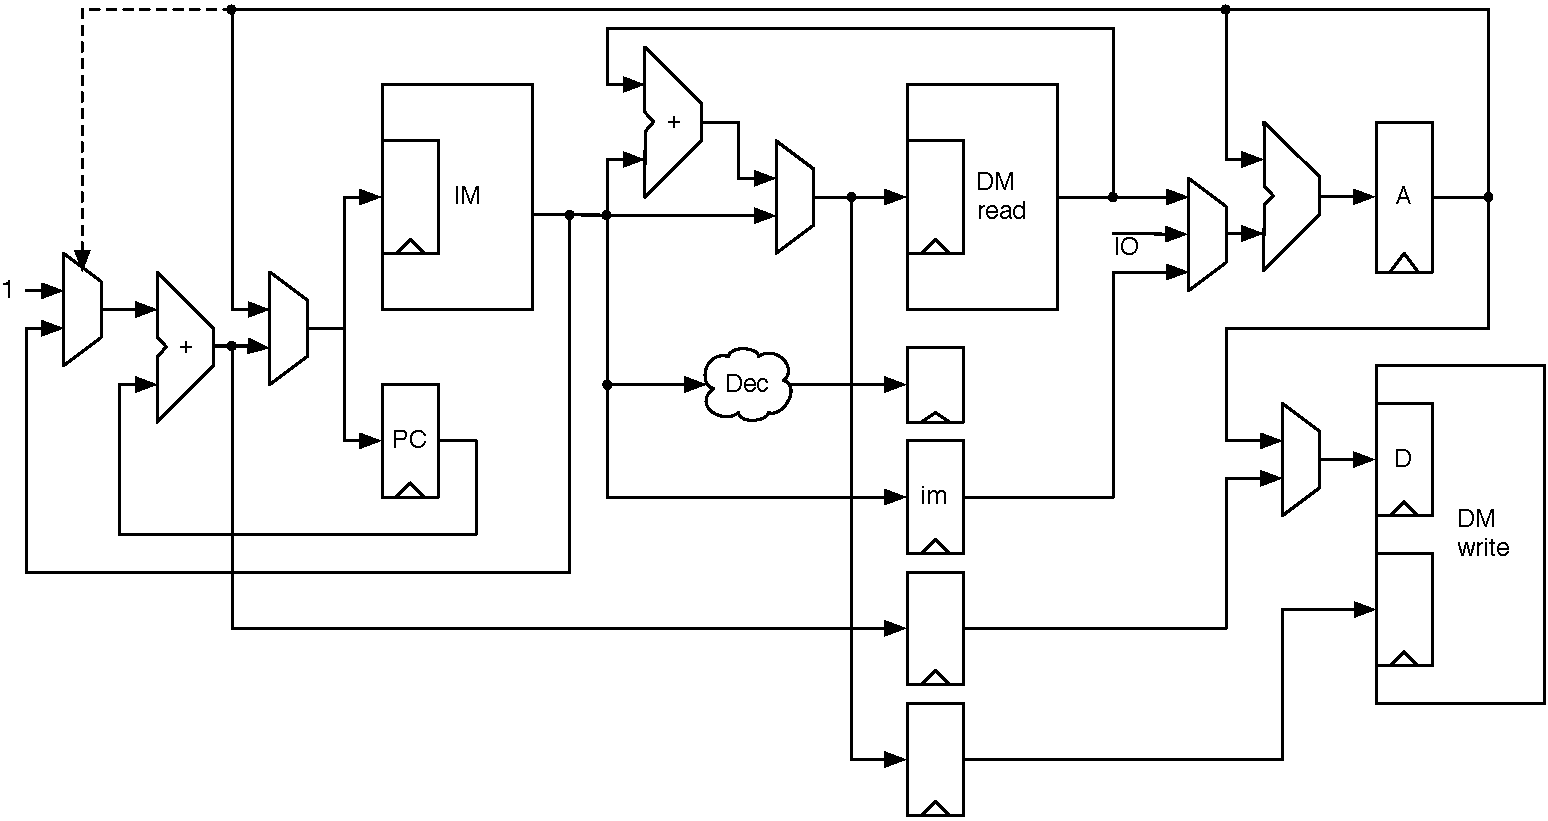
\includegraphics[width=0.8\textwidth]{fig/pipeline}
    \caption{Pipeline of the original Leros design with the fetch/decode and the read/execute/memory stages.
    There might be other pipeline configurations possible and useful.}\label{fig:pipeline}
\end{figure*}

The trend is that smaller FPGAs contain more  memory blocks in relation to the logic, about 200 LCs per memory block.
The larger devices of the Spartan-3 series increase the logic resources considerable more then the memory resources.
It is interesting to note that for Altera Cyclone chips and newer Spartan chips the relation between LCs and memory blocks stays in the range of 200 to 400 LCs per memory block independent of the device size.
Therefore we conclude that the sweet spot for a microcontroller in current FPGAs is around 300 LCs per on-chip memory block.



\section{Architectural Decisions}

To restrict the consumption of on-chip memories they are used only for the instruction memory\footnote{Very small programs can even be implemented using LCs for the instruction memory. Quartus automatically instantiates either an on-chip memory or LC based instruction memory from the same VHDL source.} and the data memory. Therefore, we avoid using additional on-chip memories for a register file. A standard register file would need two read and one write ports and therefore would consume another two on-chip memory blocks (to implement the two read ports).

Minimal resource consumption can be achieved by an accumulator design. Only a single dedicated register (the accumulator) is connected to the ALU output and provides one input to the ALU. To provide fast data locations, similar to a register file, the first 256 words in the on-chip data memory can be directly addressed for an ALU operation. Therefore, an ALU operation on two local variables takes two cycles to execute and another cycle if the result needs to written back to a local variable. This might sound expensive, but compared to the PicoBlaze and Nios~II it is not so expensive. PicoBlaze needs two clock cycles for each instruction and the economy version of Nios~II 6 clock cycles.

\chapter{Testing}

Generating LLVM code:

\begin{verbatim}
clang -S -emit-llvm x.c
\end{verbatim}

To generate test cases use \url{https://godbolt.org/} with options -emit-llvm to emit LLVM code,
which then can be compiled with \code{llc}:

In build-leros-llvm-Clang-release/bin/ you will find llc, the llvm IR compiler

\begin{verbatim}
./llc -march=leros32 triangle.ll --filetype=asm
\end{verbatim}
This should produce triangle.s, which contains the compiled function in Leros assembly language. 

an example input would be:

\begin{verbatim}
define dso_local i32 @_Z4trianglei(i32) {
  %2 = alloca i32, align 4
  %3 = alloca i32, align 4
  %4 = alloca i32, align 4
  store i32 %0, i32* %2, align 4
  store i32 1, i32* %4, align 4
  store i32 1, i32* %3, align 4
  br label %5

  %6 = load i32, i32* %3, align 4
  %7 = load i32, i32* %2, align 4
  %8 = icmp sle i32 %6, %7
  br i1 %8, label %9, label %16

  %10 = load i32, i32* %4, align 4
  %11 = load i32, i32* %3, align 4
  %12 = add nsw i32 %10, %11
  store i32 %12, i32* %4, align 4
  br label %13

  %14 = load i32, i32* %3, align 4
  %15 = add nsw i32 %14, 1
  store i32 %15, i32* %3, align 4
  br label %5

  %17 = load i32, i32* %4, align 4
  ret i32 %17
}
\end{verbatim}

\chapter{Compiler}

We have adapted the LLVM compiler~\cite{llvm:2004} for Leros, which is currently hosted at:
\url{https://github.com/leros-dev/leros-llvm}.\\
To build the compiler and related tools, clone the \texttt{leros-llvm} repository:      

\begin{verbatim}
git clone https://github.com/leros-dev/leros-llvm.git
\end{verbatim}

After cloning the repositories, the toolchain is built via. the included build script in `leros-llvm`.
\begin{verbatim}
./leros-llvm/build.sh
\end{verbatim}

The build script is directory-agnostic and can be run from anywhere. The build script will build the project in \texttt{build-leros-llvm}, which is placed next to the \texttt{leros-llvm} folder. The script will initialize and pull the submodules for \texttt{leros-clang} and \texttt{leros-lld}.\\

During the build process the build script will check out the \texttt{leros-lib} repository and place it next to the \texttt{leros-llvm} folder, wherein after finished compilation of the compiler, \texttt{crt0.leros.o} (containing the leros \texttt{\_start} procedure) as well as the Leros runtime library will be compiled and copied to the \texttt{build-leros-llvm/lib/clang/\$\{clang version\}/lib/} folder.

\texttt{build-leros-llvm/bin} will contain the LLVM binaries.\\
Add \code{path-to-repo/build-leros-llvm/bin} to your \code{PATH} variable.

\martin{Cross compiler binaries usually start with the processor name (e.g. riscv-... or patmo-clan)
to be able to distinguish between different versions. Maybe you can do so as well.}

\chapter{Leros Implementation}
\label{sec:imp}

Based on the former described design decisions, Leros is implemented in a two-stage pipeline with following visible architectural state: the program counter (PC), the accumulator register (A), the instruction memory (IM), and the data memory (DM).

\subsection{The Pipeline}

Figure~\ref{fig:pipeline} shows the pipeline of Leros. It shows the main data path, the pipeline registers, and the on-chip memories. The DM is shown twice as it is read in one pipeline stage and written in a different one. Register A is the accumulator and PC the program counter.

Leros is implemented with two pipeline stages. The first stage fetches an instruction from the IM and decodes the instruction. The second stage reads an operand from the DM and executes. In both stages the combinational logic is fed by the asynchronous output of the memory. According to our design decisions, the pipeline stage is balanced when the combinational logic (plus the routing) delay is as long as the access time of the on-chip memory.

As the input registers of on-chip memories cannot be read, the PC is duplicated. The address of the IM and the PC is either an increment of the PC by 1, an addition with a constant from the instruction (relative branch), or the content of A (indirect jump).

The read and write address of the DM is either a constant from the instruction (for the on-chip registers) or an indirection via the DM plus an offset (for loads and stores). The write data for the DM is either A for store instructions or the PC for a jump-and-link instruction to save the PC in a register.

A memory load and store uses a based register and an offset for the address. As the data memory is shared for registers and general data, load and stores are implemented by two instructions. With the first instruction the address for the register, which is used as base address for the load/store, is sent to the DM. The following instruction uses the value of the DM (the register content) and adds an offset, which is part of that instruction, to form the effective address. The data word to be written is provided by A; the result of a load is stored into A. This split of the indirect memory access into two instructions costs an additional cycle, but allows efficient reuse of the DM for registers and general data.

For on-chip memories with independent read and write port the question arises what happens on a concurrent write to and read from the same address in the same cycle. There are three options: (1) read the newly written value, (2) read the old value, or (3) undefined. The actual behavior depends on the FPGA family and is sometimes configurable. A safe way would be to forward the written result to the read output, which is in the actual version of Quartus automatically inferred (depending on the VHDL style used to describe memory). However, for an accumulator machine there is no benefit in forwarding this memory access. The last value written to DM is still in register A and can just be reused when needed by the next instruction.

\subsection{I/O Interface}

I/O read data is fed into the pipeline via the ALU. The I/O write data is the content of A. The address for the I/O instruction is part of the instruction.

The interface to I/O devices is similar to the PicoBlaze design and consists of an 8-bit I/O address, a read and write signal, and 16-bit input and output data signals. For the write instructions the address, the data, and the write signal are valid for a single cycle. For the read instruction the I/O device needs to deliver the result in the same cycle as the address and the read signal are valid. No busy or wait signals are supported. For devices with a longer access time software based polling needs to be implemented. The argument for this I/O interface is simplicity and the fact that most I/O devices already support single cycle access.


\subsection{Extensions}
%\subsection{Deadline Instruction}

One application area of Leros is a processor to implement \emph{intelligent} I/O devices. Such devices often need to generate exactly timed outputs. To simplify this timing generation a so-called \emph{deadline} instruction can be used~\cite{Edwards:06:deadline, jop:deadline}. A deadline instruction is a programmable timer with combined with the facility in the pipeline to wait cycle accurate (or in the range of a few cycles) until the timeout. With such an instruction a PWM based DA converter or a serial interface (UART) can be implemented completely in software.

For experiments with a Leros based many-core system it shall be possible to dynamically change the content of the instruction memory and the data memory. To access the shared off-chip memory a memory controller and an arbiter needs to be attached to the I/O interface. We will reuse the available components from a Java chip-multiprocessor~\cite{jop:tecs:cmp}.

To transfer instructions from the shared main memory into the instruction memory of Leros, the on-chip instruction memory needs an additional write port, which is already available (instruction fetch uses only a read port). Furthermore an instruction needs to be defined to write the content of A into the instruction memory.

We plan to use Leros for experiments with a ring-based network-on-chip~\cite{jop:csp}. With the small size of a processor node we can perform real experiments in an FPGA with a huge number of processing nodes (e.g., 100+ in the FPGA of the Altera DE2-70 board).

\subsection{Software Tools}

We started with a simple assembler written in Java with some reuse of code from the JOP project~\cite{jop:jnl:jsa2007}. Later we adapted the lexer and grammar tool ANTLR~\cite{antlr:1995} for the assembler. Using the parser generator ANTLR might sound like an overkill for the implementation of an assembler. However, the simplicity of defining a grammar enables the implementation of a  higher level assembler, which can simplify assembler programming. Furthermore, we started to retarget the muvium Java compiler\footnote{\url{http://www.muvium.com/}} for Leros. Muvium is optimized to compile simplified Java for resource-constrained microcontrollers, such as Microchip processors. Therefore, this compiler is an ideal tool for Leros.

\subsection{The Leros Regression Test Framework}

\section{Evaluation}
\label{sec:eval}

We have implemented Leros on several different FPGA boards with Altera and Xilinx FPGAs. The VHDL code of Leros is highly portable. The only changes needed for a port are the pin definitions for the board and a device specific PLL component. For the evaluation we used the free versions of Altera Quartus 10.1 and Xilinx ISE 12.4.


Table~\ref{tab:synth} shows synthesis results of Leros for different FPGA families. The last column shows the maximum clock frequency of an on-chip memory of that FPGA family. We have selected the fastest speed grade for all devices for this table. To derive the maximum clock frequencies for the Leros design and the on-chip memory, the designs use a PLL and have been over-constraint with a high clock frequency.
From the table we see that we have achieved our goals to build a small processor with a maximum clock frequency in the range of half the on-chip memory clock frequency. In the benchmarked configuration Leros consumes only a single on-chip memory. This can be explained by the small test program (a LED blinking at 0.5 Hz, implemented by 36 instructions) where the ROM is implemented in logic cells instead of an on-chip memory.


\begin{table}
\small
\centering 
\caption{Synthesis results of Leros for different FPGAs}
\label{tab:synth}
\begin{tabular}{rrrrr}
\toprule
 & Logic & Memory & Fmax & BRAM Fmax \\
 FPGA & (LC) & (blocks) & (MHz) & (MHz) \\
\midrule
Cyclon & 195 & 1 & 132 & 256 \\
Cyclon II & 190 & 1 & 146 & 235 \\
Cyclon III & 188 & 1 & 150 & 315 \\
Cyclon IV & 189 & 1 & 160 & 315 \\
Spartan-3E & 188 & 1 & 129 & 297 \\
Spartan-6 & 112 & 1 & 182 &  320 \\
\bottomrule
\end{tabular}
\end{table}

%On the Spartan devices both the ROM and the data memory are implemented in block RAMs. Therefore, the logic count is smaller than in the Altera devices. 

The Spartan-6 device contains 6-bit LUTs and therefore the LC count is lower. Furthermore, the available 16 Kbit BRAM is logically split into two 8 Kbit memories for the instruction and data memory.


We compare Leros with PicoBlaze on the Nexys2 FPGA board, which contains a Spartan XC3S500E-4. Both processors contain an interface to the LEDs and buttons and use a PLL (DCM) to clock the processor at 100~MHz. To report the maximum clock frequency we over-constrained the design by generating a 150~MHz clock with the PLL.
For the comparison of Leros with PicoBlaze we wrote a minimalistic embedded application: a light control. The light control uses a LED on the FPGA board as output and can be switched with one button between three states (off, dimmed, on). Dimming of the LED is generated by pulse width modulation (PWM) in software.

\todo{PicoBlaze: 40 words of 18 bit for the dimmer -- report program size for both.}
\todo{Reduce: Leros on-chip memory....}

Table~\ref{tab:comp} shows the resource utilization and maximum clock frequency of the design for a Spartan-3E device.\footnote{The maximum clock frequency is slightly lower as in Table~\ref{tab:synth}, as the FPGA on the Nexys2 board is a slower speed grade.} Leros is comparable in resource consumption and maximum clock frequency with PicoBlaze. However, Leros implements a 16-bit data path and can execute an instruction in a single cycle, whereas PicoBlaze is a 8-bit processor and needs 2 clock cycles for each instruction.
%
%The SpartanMC is a processor for a slightly different design point.
%In~\cite{SpartanMC:2007} SpartanMC is compared against 32-bit RISC cores, such as LEON-II and MicroBlaze.
In contrast to Leros, SpartanMC implements a register machine and needs therefore more resources. Compared to PicoBlaze, SpartanMC executes basic operations in a single cycle. The lower clock frequency of SpartanMC is due to the usage of two phase-shifted clocks for the sub-dividing of two pipeline stages into two phases.



The implementation of Leros on several FPGA boards and the comparison with PicoBlaze shows that we have achieved our design goal of a small, fully pipelined processor, which can be clocked at a reasonable frequency. Except for the PLL component, all VHDL sources are vendor agnostic. This experiments also shows that usage of vendor specific components, as done in the PicoBlaze design, have minimal, or perhaps no, impact on the achievable size and performance. Current synthesize tools are mature enough to infer a good hardware implementation from carefully written VHDL code.

\begin{table}
\small
\centering 
\caption{Comparison of Leros with PicoBlaze and SpartanMC on a Spartan XC3S500E-4}
\label{tab:comp}
\begin{tabular}{rrrr}
\toprule
 & Logic & Memory & Fmax \\
 Processor & (LC) & (blocks) & (MHz) \\
\midrule
Leros & 188 & 1 & 115 \\
PicoBlaze & 177 & 1 & 117 \\
SpartanMC & 1271 & 3 & 50 \\
\bottomrule
\end{tabular}
\end{table}
\todo{Add a JOP microcode version into the table.}

\todo{For the final version update the numbers with the actual (finished) implementation of Leros.}

\section{Conclusion}
\label{sec:conclusion}

This paper presents the design and implementation of a tiny microcontoller for FPGAs. Leros is a pipelined processor, optimized to balance the resource consumption between logic cells and on-chip memory. The 16-bit processor Leros consumes less than 200 logic cells and 1--2 on-chip memories.
To achieve optimal timing, the combinational logic and routing resource delays are designed to be equal to the access time of on-chip memories. Therefore, the maximum clock frequency of Leros is in the range of half of the maximum clock frequency of on-chip memories. This tiny processor is an ideal choice for utility functions, such as implementing an intelligent peripheral component for an SoC. Due to the small size it can also be used for research on many-core architectures in medium sized FPGAs.

% We have implemented a XXX core multiprocessor system with Leros in the low-cost FPGA Cyclon-II with 70.000 LCs and XXX on-chip memories. This example system can be clocked at 140~MHz.

\section*{Source Access}

The Leros design is open source and available from \url{https://github.com/schoeberl/leros}. The distribution currently supports following FPGA boards directly: Altera DE2-70, Nexys2, and Cycore. As the interface to the off-chip world is minimal (clock, buttons, and LEDs), a port to a different FPGA board is trivial.


\section{Conclusion}
\label{sec:conclusion}

\todo{Rephrase what this paper is about and list the main contributions and results.}

\subsection*{Acknowledgment}

\todo{Sometimes we received some help. Sometimes external funding.}



\bibliographystyle{plain}
% Please do not add any references to msbib.bib.
% They get lost when I 'generate' is again (see Makefile)
\bibliography{other,msbib}

\end{document}
